\section{Integrators: Explicit Runge-Kutta 4}
A common explicit RK4-scheme is given as:
\begin{align}
    \dot{x} &= F(x,u)\\
    x_{k+1} &= x_k +\frac{h}{6}k_1 + 2k_2 + 2k_3 + k_4\\
\end{align}
With $k$'s given by:
\begin{align}
    k_1 &= F(x_k, u_k)\\
    k_2 &= F(x_k + \frac{h}{2}k_1, u_k)\\
    k_3 &= F(x_k + \frac{h}{2}k_2, u_k)\\
    k_4 &= F(x_k + hk_3, u_k)\\
\end{align}


Yielding the following buther-tableau:
\begin{table}[h]
    \centering
    \begin{tabular}{c|cccc}
         0 & & &  \\
         $\frac{1}{2}$& $\frac{1}{2}$ & &\\ $\frac{1}{2}$& 0 & $\frac{1}{2}$ & &\\
         1 & 0 & 0 & 1 &\\
         \hline &
         $\frac{1}{3}$ & $\frac{1}{6}$ & $\frac{1}{6}$ & $\frac{1}{3}$ 
         
    \end{tabular}
    \caption{RK4 butcher tableau}
    \label{tab:my_label}
\end{table}

Figure \ref{fig:RK4_Stability} shows the stability region of explicit runge-kutta methods.

\begin{figure}[h]
    \centering
    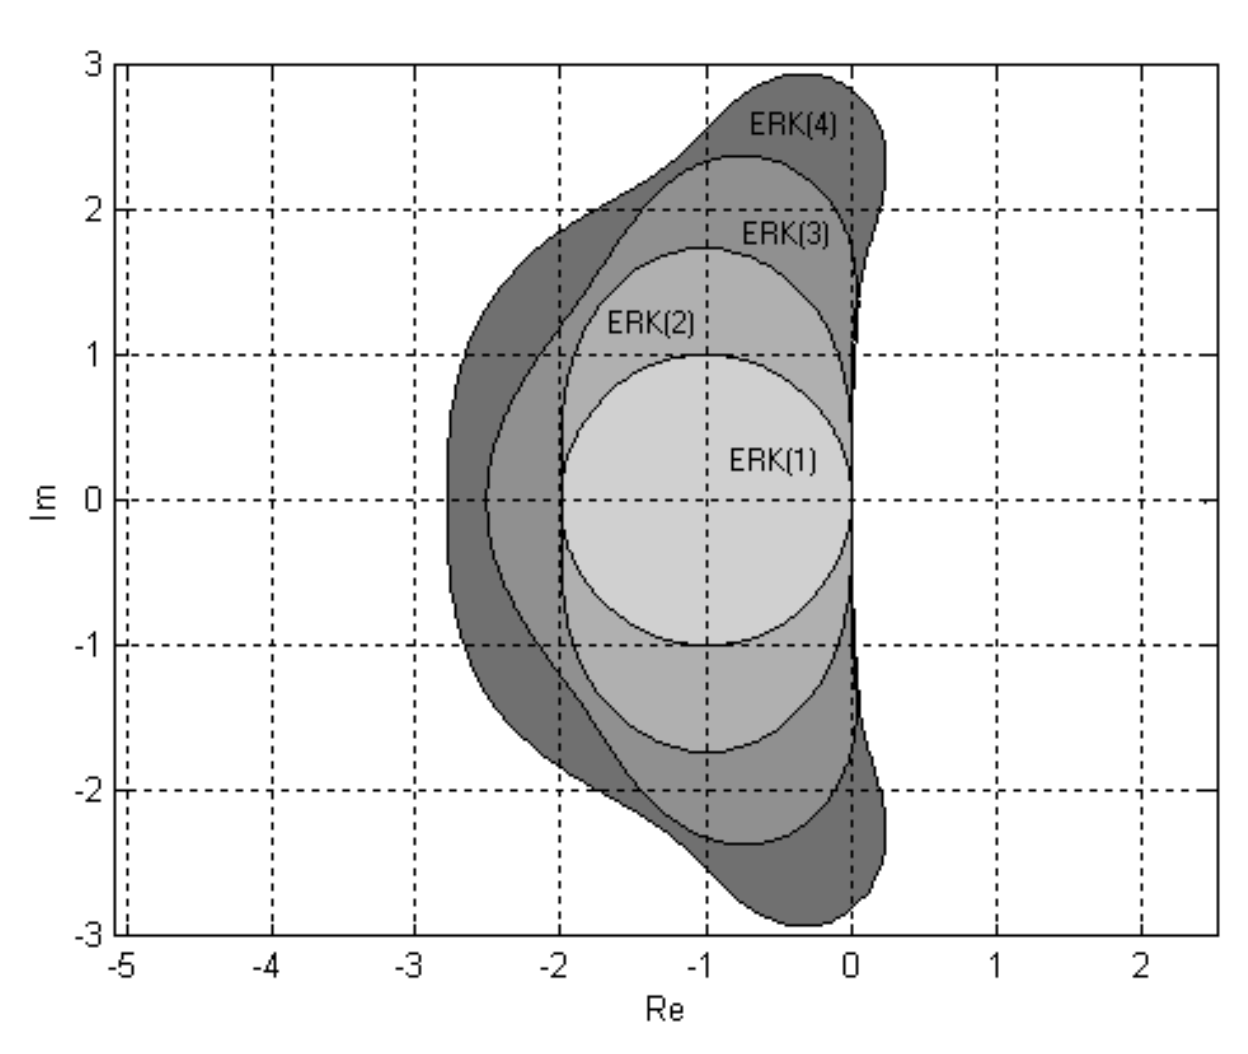
\includegraphics[width=0.8\textwidth]{Figures/RK_Stability_Region.PNG}
    \caption{Runge-Kutta stability regions[\cite{ModSimAuto}]}
    \label{fig:RK4_Stability}
\end{figure}

The bilinear SIR-model will have unstable regions which require the integrator step length to be set sufficiently low in order to get accurate steps.

\subsection{Sensitivities}


\subsubsection{Variational Approach}
General state and input sensitivities can be calculated from partial derivatives of the ODE:
\begin{align}
    \dot{A}(t) &= \frac{\partial F}{\partial x}|_{x(t),u_k} A(t), & &A(t_k) = I\label{eq:sens_A}\\
    \dot{B}(t) &= \frac{\partial F}{\partial x}|_{x(t), u_k} B(t) + \frac{\partial F}{\partial u}|_{x(t), u_k}, & &B(t_k) = 0 \label{eq:sens_B}
\end{align}
Where the ODE for state sensitivity $A(t)$ contains one term, while ODE for input sensitivity $B(t)$ contains two terms due to $u_k$'s indirect impact on $F(t, x, u)$ through $x$. Implementing sensitivities using the variational approach will yield additional integration errors in the extra ODEs (compared to algorithmic differentiation).

\subsubsection{Algorithmic Differentiation}
In algorithmic differentiation, the problem is first discretized, then the sensitivities are obtained from the resulting algorithm. This effectively limits the integration error of the sensitivities to some magnitude of the state integration error.
\begin{algorithm}[H]
\SetAlgoLined
\KwData{$x_k, u_k, h, N$}
 \For{$i$ = 0 : $N-1$}{
    $k_1 = F(x_k, u_k)$\\
    $k_2 = F(x_k + \frac{h}{2}k_1, u_k)$\\
    $k_3 = F(x_k + \frac{h}{2}k_2, u_k)$\\
    $k_4 = F(x_k + hk_3, u_k)$\\
   $x_{k+1} = x_k + \frac{h}{6}k_1 + 2k_2 + 2k_3 + k_4$\\
 }
 \caption{RK4 Integration Algorithm}
\end{algorithm}
The sensitivity equations can be derived using equations \ref{eq:sens_A} and \ref{eq:sens_B}. With full state trajectories provided, the sensitivities can be calculated afterwards according to algorithm \ref{alg:RK4_sense}.

\begin{algorithm}[H]
\SetAlgoLined
\KwData{$[x_0, \dots, x_N], [u_0, \dots, u_N], h, N$}
 \For{$i$ = 0 : $N-1$}{
    $C_x = \frac{\partial}{\partial x}(\frac{h}{6}k_1 + 2k_2 + 2k_3 + k_4)|_{x_k, u_k})$\\
    $C_u = \frac{\partial}{\partial u}(\frac{h}{6}k_1 + 2k_2 + 2k_3 + k_4)|_{x_k, u_k})$\\
    $A_{k+1} = (I + C_x) A_k$\\
    $B_{k+1} = (I + C_x) B_k + C_u B_k$}
 \caption{RK4 Sensitivity Calculation}
 \label{alg:RK4_sense}
\end{algorithm}

Here, the evaluation points are updated with the integrated state, which results in different sensitivity errors than the variational approach. For the upcoming SIR-model, the algorithm will be implemented to yield sensitivities iteratively with the integration.

\subsubsection{Implementation on the SIR-model}
Both approaches require partial derivatives of the SIR-ODE:
\begin{align}
    \frac{\partial F}{\partial x} &= \frac{\partial 
    \begin{bmatrix}
    \frac{-u x_1 x_2}{N_{pop}}\\
    \frac{u x_1x_2}{N_{pop}} - \alpha x_2\\
    \alpha x_2
    \end{bmatrix}
    }{\partial x} = \begin{bmatrix}
    -\frac{ux_2}{N_{pop}} & -\frac{ux_1}{N_{pop}} & 0\\
    \frac{ux_2}{N_{pop}} & \frac{ux_1}{N_{pop}} - \alpha & 0\\
    0 & \alpha & 0
    \end{bmatrix}
    \label{eq:dFdx_SIR}\\
    \frac{\partial F}{\partial u} &= \frac{\partial 
    \begin{bmatrix}
    \frac{-u x_1 x_2}{N_{pop}}\\
    \frac{u x_1 x_2}{N_{pop}} - \alpha x_2\\
    \alpha x_2
    \end{bmatrix}
    }{\partial u} = 
    \begin{bmatrix}
    \frac{-x_1 x_2}{N_{pop}}\\
    \frac{x_1 x_2}{N_{pop}}\\
    0
    \end{bmatrix}
    \label{eq:dFdu_SIR}
\end{align}

Using equations \ref{eq:dFdx_SIR} and \ref{eq:dFdu_SIR}, the two approaches for sensitivity were implemented with the RK4 scheme in Python.

\begin{figure}[h]
    \centering
    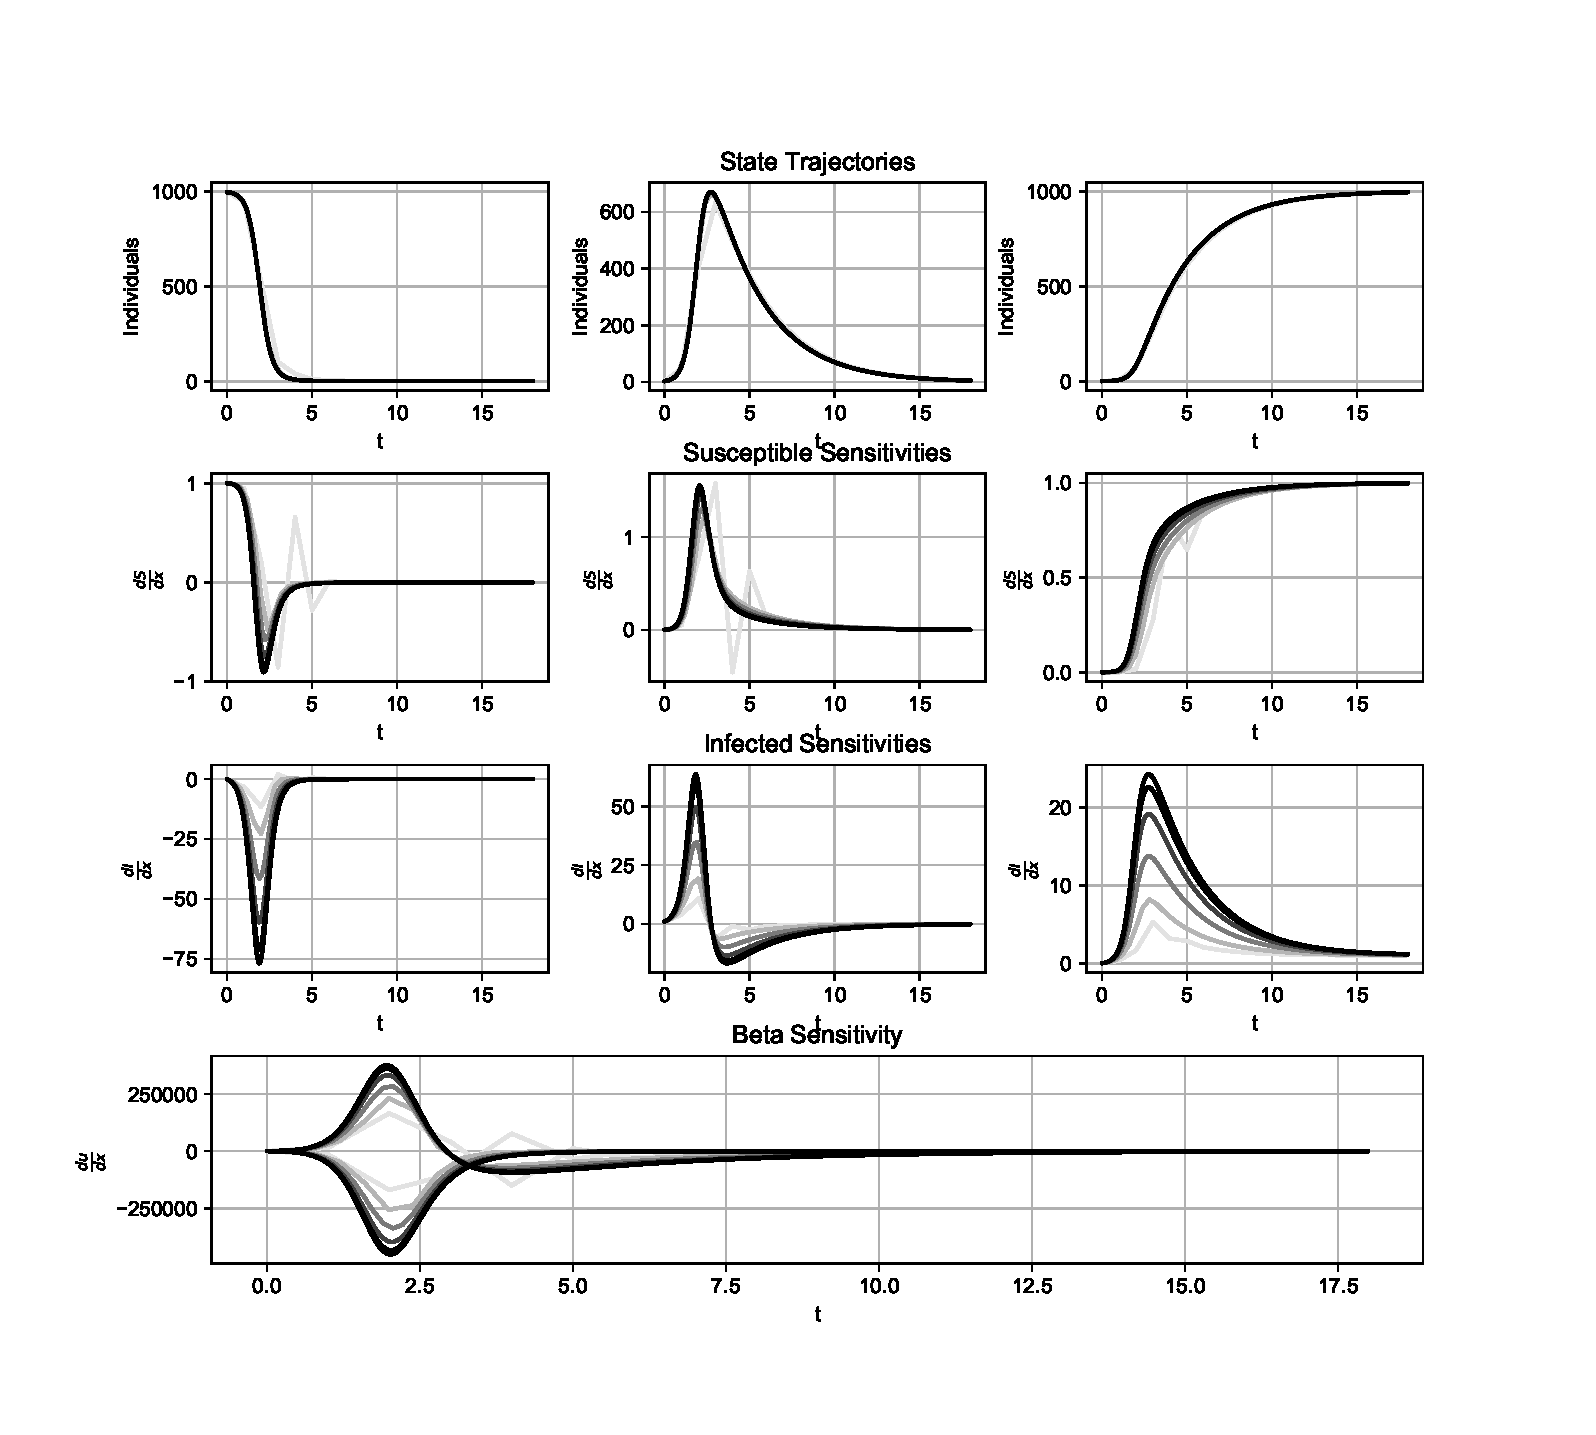
\includegraphics[width=.9\linewidth]{Figures/Autodiff_Sensitivities.eps}
    \caption{RK4-scheme sensitivities and trajectories with autodifferentiation. $\Delta t = [1.        , 0.39810717, 0.15848932, 0.06309573, 0.02511886,
       0.01      ]$ gradually colored from white to black}
    \label{fig:RK4_Autodiff}
\end{figure}

The susceptible and infected sensitivities with respect to the susceptible and infected populations (plots $[1:2,1:2]$) show that the most fragile timepoints of the epidemic occurs when the product of susceptibles and infected are highest. The third column shows sensitivities with respect to the recovered individuals.

Even though automatic differentiation should present a smaller integration error, it was not possible to find visible differences between the two approaches using stepsizes down to $\Delta t = 1e-5$. When compared to the 'true' trajectories, they presented the same errors.
\newpage
\subsection{Bounds and Nonlinearity}
The SIR-model itself is a Lipschitz, continously differentiable ODE which with the variational RK4-scheme approach also has continous dynamics for the sensitivities. It is visible in figure \ref{fig:RK4_Autodiff} that the maximum sensitivities of the susceptible and infected states are found at $S = I$ for $\mathscr{R}_0 > 1$.
\todo{Add more}
\iffalse
\begin{align}
        &\frac{\partial F}{\partial x}|_{x(t),u_k} A(t) = 0\\
 &\frac{\partial F}{\partial x}|_{x(t), u_k} B(t) + \frac{\partial F}{\partial u}|_{x(t), u_k} = 0
\end{align}

State $R$ can be excluded from the analysis, yielding a $2\times 2$ analysis:

\begin{equation}
\frac{\partial F}{\partial x}|_{x(t),u_k} A(t) = 
\begin{bmatrix}
    a_{12}\,u\,x_{2}-a_{11}\,u\,x_{1} & -a_{12}\,\left(\alpha-u\,x_{1}\right)-a_{11}\,u\,x_{1}\\ a_{22}\,u\,x_{2}-a_{21}\,u\,x_{2} & -a_{22}\,\left(\alpha-u\,x_{1}\right)-a_{21}\,u\,x_{1} 
    \end{bmatrix}
\end{equation}
Inserting the 


\subsubsection{Instability and Step Length}
As shown in \ref{ch:SIR_stability} the SIR-model will have local unstable dynamics, which in turn cause unstable integration errors. The errors will have to be restricted using small enough integration steps. The instability of the integrator can be determined by:
\begin{equation}
    R_{E, max}(\lambda \Delta t) = det[I-\text{Re}_{max}[\lambda_{1,2}] \Delta t(A - 1b^T)]
\end{equation}
Where $A$ and $b$ is given by the buther tableau. Inserting the eigenvalue corresponding to the most unstable dynamic achieveable, this yields:
\begin{equation}
    R_{E, max}(\lambda \Delta t) = det[I- \frac{\beta_{max}(S_0-I_0) - \alpha}{2N} \Delta t(A - 1b^T)]
\end{equation}
\fi
\subsection{Integrators: Collocation}
A collocation integrator constructs the trajectory using
parameters $\theta$ on a time grid of $d+1$ points in $[t_k, t_{k+1})$ ($[\tau_0, \tau_1, \dots, \tau_d]$). Parameters $theta$ are constrained to equal the value of the trajectory at these points, giving the full trajectory as a sum of lagrange polynomials:
\begin{align}
    P_i(\tau) &= \prod_{j=0, j \neq i}^{d+1} \frac{\tau-\tau_j}{\tau_i - \tau_j}\\
    s_k(\theta, \tau) &= \sum_{j=0}^{d+1} \theta_j P_j(\tau)
\end{align}
Matrices $C \in \mathbb{R}^{(d+1)\times(d+1)}$ and $B, D \in \mathbb{R}^{(d+1)}$ can be constructed, respectively containing coefficients for the derivatives and the end state for the polynomials. This makes it possible to calculate $\bm{\theta}$, $\bm{\dot{\theta}}$ and the objective value accumulated over each timestep $t_k$. Figure \ref{fig:Lagrange_Polynomials} illustrates the properties of the coefficients.

\begin{figure}[h]
    \centering
    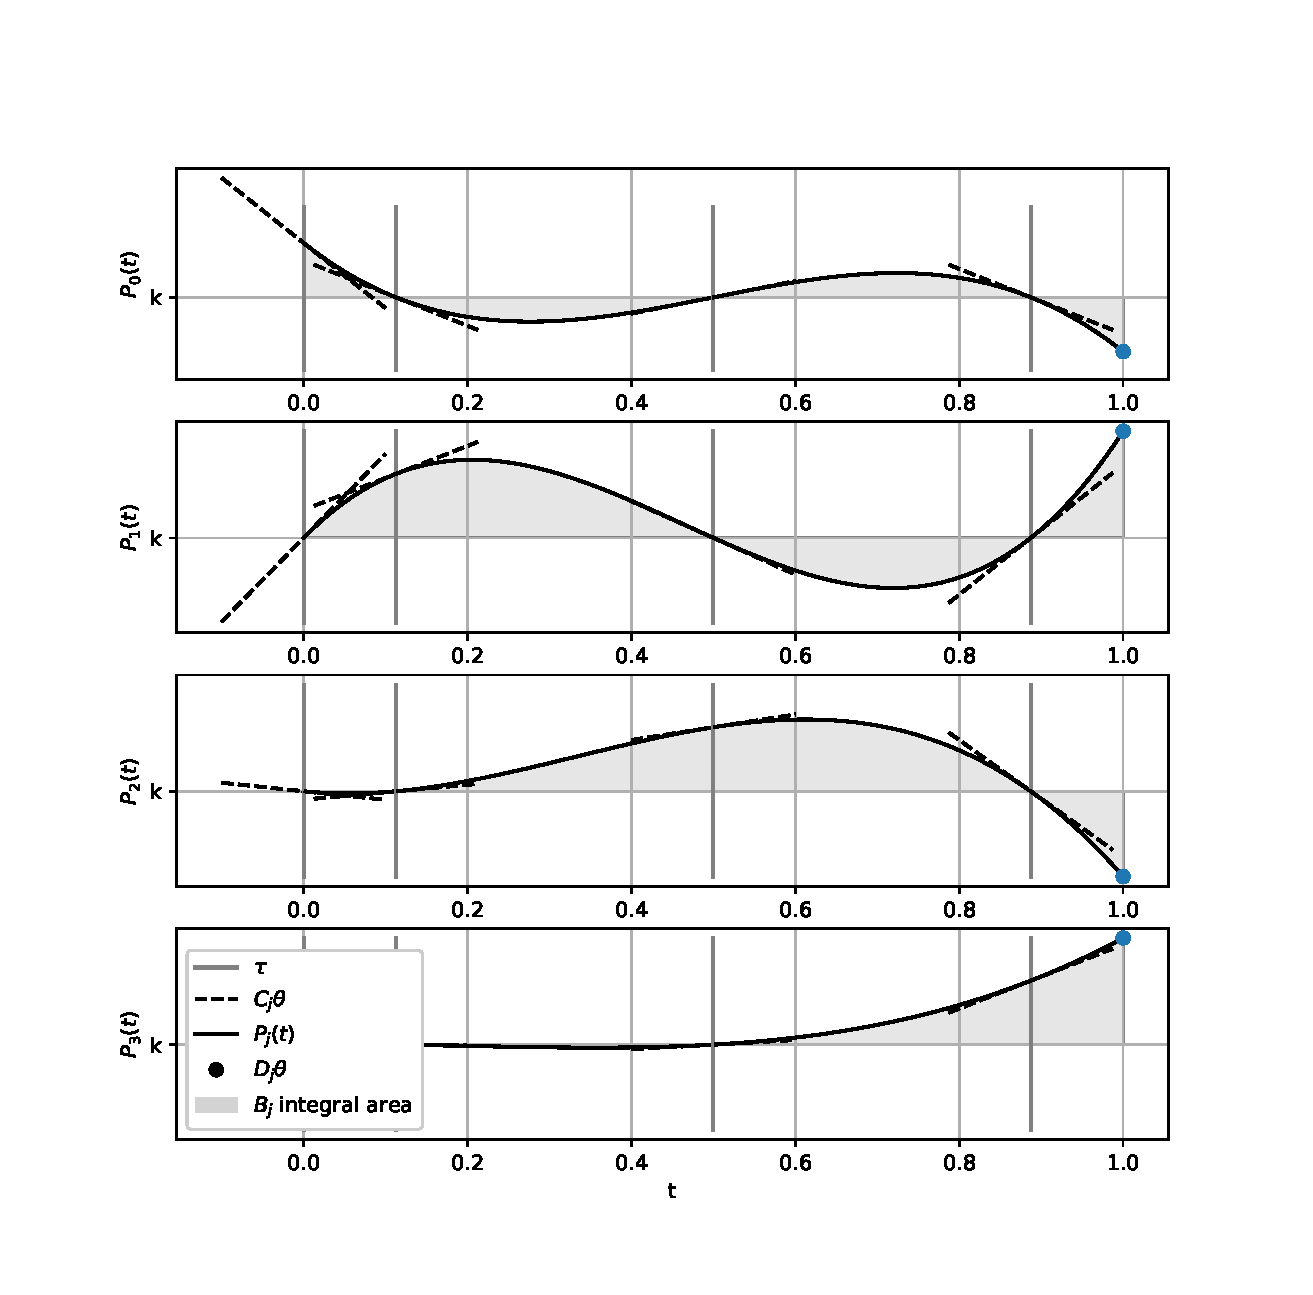
\includegraphics[width=1\textwidth]{Figures/lagrange_polynomial.eps}
    \caption{Lagrange Polynomials using legendre-timepoints for $d=3$}
    \label{fig:Lagrange_Polynomials}
\end{figure}

The derivative of the trajectory can be constrained to match the ODE in order to approximate the true trajectory at the chosen timepoints:
\begin{align}
    g_{\text{col}} &= \dot{s}_k(\theta, \tau) - F(\theta_i, t_k + \tau_i) = \sum_{j=0}^{d+1}\theta_j\dot{P}_j(t_k + \tau_i)  - F(\theta_i, t_k + \tau_i) = 0\\ \forall k, i &\in [0,\dots, N-1], [0, \dots d]\nonumber
\end{align}
\subsubsection{Sensitivities}
$g_{col} = 0$ can be solved with newton-raphson, yielding $\frac{\partial g_{col}}{\partial \theta}$ as a biproduct. The sensitivities of the integrator with respect to state and control input can be derived from the implicit function theorem, yielding:
\begin{align}
    \frac{\partial \theta}{\partial x} &= \frac{\partial g_{col}}{\partial \theta}^{-1}\frac{\partial g_{col}}{\partial x} &     \frac{\partial \theta}{\partial u} &= \frac{\partial g_{col}}{\partial \theta}^{-1}\frac{\partial g_{col}}{\partial u}
\end{align}



